\section{持久化}
    \subsection{概念}
    持久化的概念就是保存所有版本,像是我們用電腦時常常使用的
    \verb|ctrl+z|。

    想想如果我們要問第k次操作後的某段區間,我們有兩種已知做法。

    \begin{enumerate}
        \item 對詢問的k做排序,依序處理完再重排輸出。
        \item 用n棵線段樹,但會花費過多空間。
    \end{enumerate}

    而持久化就是讓我們可以用最小的空間,備份所有版本。
    以線段樹而言就可以用共用節點的方式進行。

    \begin{figure}[!htbp]
        \centering
        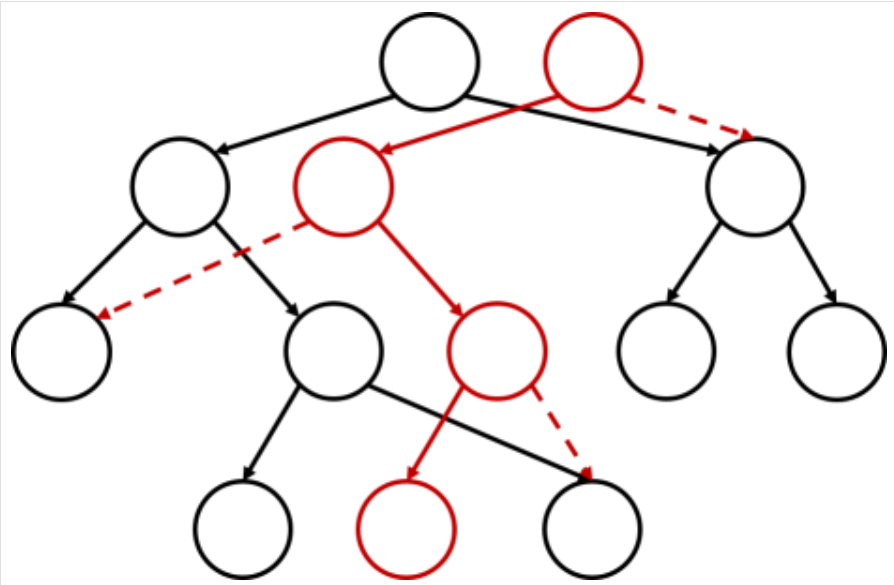
\includegraphics[width=0.8\textwidth]{../Images/SEG3.png}
    \end{figure}

    \subsection{實作}

\begin{lstlisting}[caption=持久化線段樹]
struct node{
    node *lch,*rch;
    int val;
    
    node(){
        lch=rch=nullptr;
        val=0;
    }
    
    void pull(){
        val=lch->val + rch->val;
    }
};

void build(int l,int r,node *&p){
    p=new node();
    if(l==r) return;
    int mid=(l+r)>>1;
    build(l,mid,p->lch);
    build(mid+1,r,p->rch);
    p->pull();
}

void modify(int pos,int val,int lb,int rb,node *pre,node *&cur){
    // 對於有改變的節點開新的
    cur=new node();
    
    if(lb==rb){
        cur->val=pre->val+val;
        return;
    }
    
    // 共用節點
    cur->lch=pre->lch;
    cur->rch=pre->rch;
    int mid=(lb+rb)>>1;
    
    if(pos<=mid) modify(pos,val,lb,mid,pre->lch,cur->lch);
    if(mid<pos) modify(pos,val,mid+1,rb,pre->rch,cur->rch);
    
    cur->pull();
}

int query(int l,int r,int lb,int rb,node *ver){
    if(l<=lb && rb<=r) return ver->val;
    
    int ret=0;
    int mid=(lb+rb)>>1;
    if(l<=mid) ret+=query(l,r,lb,mid,ver->lch);
    if(mid<r) ret+=query(l,r,mid+1,rb,ver->rch);
}
\end{lstlisting}

    \subsection{範例與練習}

    \example 洛谷P3834 【模板】可持久化線段樹 2

    \textbf{題目敘述}

    這是一個非常經典的可持久化權值線段樹入門題——靜態區間第 $k$ 小。

    數據已經過加強,請使用可持久化權值線段樹。同時請注意常數優化。

    給定 $n$ 個整數構成的序列 $a$,對於指定的閉區間 $[l, r]$ 查詢其區間內的第 $k$ 小值。

    \textbf{輸入說明}

    第一行包含兩個整數,分別表示序列的長度 $n$ 和查詢的個數 $m$。
    
    第二行包含 $n$ 個整數,第 $i$ 個整數表示序列的第 $i$ 個元素 $a_i$。
    
    接下來 $m$ 行每行包含三個整數 $ l, r, k$ ,表示查詢區間 $[l, r]$ 內的第 $k$ 小值。

    $1 \leq n,m \leq 2\times 10^5$,$|a_i| \leq 10^9$,$1 \leq l \leq r \leq n$,$1 \leq k \leq r - l + 1$

    \textbf{輸出說明}

    對於每次詢問,輸出一行一個整數表示答案。

    \textbf{範例測試}

    \begin{tabular}{|m{7cm}|m{7cm}|}
        \hline
        範例輸入 1 & 範例輸出 1 \\
        \hline
        \verb|5 5|  & \verb|6405| \\
        \verb|25957 6405 15770 26287 26465|  & \verb|15770| \\
        \verb|2 2 1|  & \verb|26287| \\
        \verb|3 4 1|  & \verb|25957| \\
        \verb|4 5 1|  & \verb|26287| \\
        \verb|1 2 2|  & \\
        \verb|4 4 1|  & \\
        \hline
    \end{tabular}

    \textbf{持久化線段樹作法}

    我們需要使用值域線段樹,存放每個數字出現過幾次,並使用持久化操作,記錄所有版本,
    從左到右第N個版本就是區間$[1,N]$的線段樹。

    如此一來,我們就可以執行查詢了,查詢時,我們想要找到第k小的數,而第k小的數字有一個特點,
    他大於前面的洽好$k-1$個數,所以我們可以在線段樹上做二分搜,如果他已經比超過k個數字大了,
    就找小一點的數字,反之則找大一點的數字。

    接者,因為值域很大,所以我們可以考慮做離散化,而不是用動態開點(因為時間卡的很緊)。

\begin{lstlisting}[caption=區間第k小題解]
struct node{
    node *lch,*rch;
    int val;
    
    node(){
        lch=rch=nullptr;
        val=0;
    }
    
    void pull(){
        val=lch->val + rch->val;
    }
};

void build(int l,int r,node *&p){
    p=new node();
    if(l==r) return;
    int mid=(l+r)>>1;
    build(l,mid,p->lch);
    build(mid+1,r,p->rch);
    p->pull();
}

void modify(int pos,int lb,int rb,node *pre,node *&cur){
    // 對於有改變的節點開新的
    cur=new node();
    
    if(lb==rb){
        cur->val=pre->val+1;
        return;
    }
    
    // 共用節點
    cur->lch=pre->lch;
    cur->rch=pre->rch;
    int mid=(lb+rb)>>1;
    
    if(pos<=mid) modify(pos,lb,mid,pre->lch,cur->lch);
    if(mid<pos) modify(pos,mid+1,rb,pre->rch,cur->rch);
    
    cur->pull();
}

int query(int val,int lb,int rb,node *l,node *r){
    if(lb==rb) return lb;
    int k=r->lch->val - l->lch->val;
    int mid=(lb+rb)>>1;
    if(val<=k) return query(val,lb,mid,l->lch,r->lch);
    else return query(val-k,mid+1,rb,l->rch,r->rch);
}

int main(){
    // input
    for(int i=0;i<n;++i){
        modify(v[i],1,mxn,ver[i],ver[i+1]);
    }
    
    int l,r,k;
    while(m--){
        // input 查詢範圍與 k
        query(k,1,mxn,ver[l-1],ver[r])-1;
    }
}
\end{lstlisting}

    \problem 洛谷P4587 [FJOI2016]神秘數

    \textbf{題目敘述}

    一個可重複數字集合 $S$ 的神秘數定義為最小的不能被 $S$ 的子集的和表示的正整數。例如 $S={1,1,1,4,13}$,有:$1 = 1$,$2 = 1+1$,$3 = 1+1+1$,$4 = 4$,$5 = 4+1$,$6 = 4+1+1$,$7 = 4+1+1+1$。

    $8$ 無法表示為集合 $S$ 的子集的和,故集合 $S$ 的神秘數為 $8$。

    現給定長度為 $n$ 的正整數序列 $a$,$m$ 次詢問,每次詢問包含兩個參數 $l,r$,你需要求出由 $a_l,a_{l+1},\cdots,a_r$ 所組成的可重集合的神秘數。

    \textbf{輸入說明}

    第一行一個整數 $n$,表示數字個數。
    第二行 $n$ 個正整數,從 $1$ 編號。
    
    第三行一個整數 $m$,表示詢問個數。
    接下來$m$行每行包含兩個整數$l,r$。

    $1\le n,m\le {10}^5$,$\sum a\le {10}^9$

    \textbf{輸出說明}

    對於每次詢問,輸出一行對應的答案。

    \textbf{範例測試}

    \begin{tabular}{|m{7cm}|m{7cm}|}
        \hline
        範例輸入 1 & 範例輸出 1 \\
        \hline
        \verb|5|  & \verb|2| \\
        \verb|1 2 4 9 10|  & \verb|4| \\
        \verb|3|  & \verb|8| \\
        \verb|1 1|  & \\
        \verb|1 2|  & \\
        \verb|1 3|  & \\
        \hline
    \end{tabular}